\subsection{A Survey of Statistical User Simulation Techniques for Reinforcement-Learning of Dialogue Management Strategies \cite{Schatzmann2006}}

This paper briefly summarizes the role of the dialogue manager in a \emph{Spoken Dialogue System (SDS)}, gives a short introduction to reinforcement-learning of dialogue management strategies and reviews the literatures on user modelling for simulation-based strategy learning. It further describes recent work on user model evaluation and discusses some of the current research issues.
\begin{figure}[h]
  \centering
  % Requires \usepackage{graphicx}
  \includegraphics[width=.6\linewidth]{khan2004-dm.png}\\
  \caption{learning dialogue strategies with a simulated user}\label{fig:khan04-dm}
\end{figure}

In SDS, the task of the \emph{dialogue Manager (DM)} is to control the flow of the dialogue and to decide which actions to take in response to user input. Specifically, DM needs a \emph{dialogue strategy} that defines when to take the initiative, when to confirm receipt, and so forth. An interesting approach to learn such strategies is through training a statistical, predictive user model for simulating user responses, which can then be used to learn the desired dialogue strategies through trial-and-error interactions (cf. Figure \ref{fig:khan04-dm}).

The second and third sections of the paper discuss  the role of the dialogue management and the reinforcement technique. Since these topics are already covered in other relevant summaries, we choose not to present them here.

Compared with the early rule-based approaches for user modelling, statistical user models are more appealing for the following reasons: 1) The purpose of the user model is not to capture the individual characteristics of a specific user, but to form the basis of a user simulation tool, so it needs to represent the statistical distribution over all types of user behaviour and user responses. These requirements clearly favour a statistical approach; 2) The second advantage of statistical models is that the model parameters can be estimated using real human-computer dialogue data. 3) The user model is also likely to be more robust, more scalable and easier to port to a different domain or dataset. The paper then summaries the recent statistical models into the following groups:

\textbf{N-grams} This method introduces a simple n-gram model for predicting the user action $\hat{a}_{u,t}$ at time $t$ that is most probable given the dialogue history of system and user actions. The weakness of the early bigram model is that it does not place any constraints on the simulated user behaviour. The bigram model is modified to predict only ``sensible'' user responses in some later work, but it still doest not ensure consistency over the course of a dialogue, because of the flawed assumption that every user response depends only on the previous system turn.

\begin{figure}[h]
  \centering
  % Requires \usepackage{graphicx}
  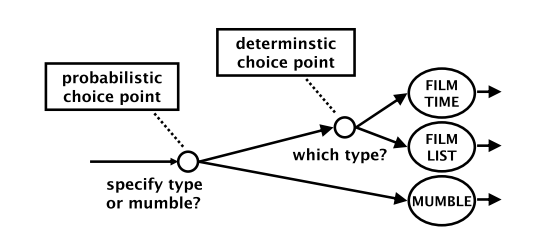
\includegraphics[width=.6\linewidth]{khan2004-graph.png}\\
  \caption{An example of the graph-based approach}\label{fig:khan04-graph}
\end{figure}

\textbf{Graph-based Models} This method combines deterministic rules for goal-dependent actions and probabilistic modelling to cover the conversational behaviour of the simulated user. An example model is shown in Figure \ref{fig:khan04-graph}, in which the arcs of the network represent actions and the nodes represent choice points. Some of the choice points are identified as probabilistic, representing a random decision by the simulated user. The major disadvantage is the high dependence on domain-specific knowledge, and the identification of probabilistic/deterministic choice points requires manual effort.

\begin{figure}[h]
  \centering
  % Requires \usepackage{graphicx}
  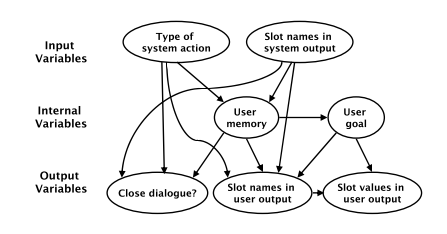
\includegraphics[width=.6\linewidth]{khan2004-bayesian.png}\\
  \caption{An example of the Bayesian Network approach}\label{fig:khan04-bayesian}
\end{figure}


\textbf{Bayesian Networks} The goal of this approach is to avoid the manual effort involved in building networks of choice points, while ensuring that actions are consistent with the user's goal. Figure \ref{fig:khan04-bayesian} shows an example of the network. It is suggested that the network can be easily extended to include factors such as the level of cooperativeness, the degree of initiative, etc.

\textbf{Machine-Learning Techniques} Recent work by Georgila et al. \cite{Georgila2005} returns to Markov models and explores the use of richer state descriptions, longer dialogue histories and machine-learning techniques. They use linear feature combination to map from a state $s$ to a vector of real-valued features $f(s)$. Supervised learning is then used to estimate a set of weights which describe how useful each vector element of $f(s)$ is for predicting an action $a$.

\begin{figure}[h]
  \centering
  % Requires \usepackage{graphicx}
  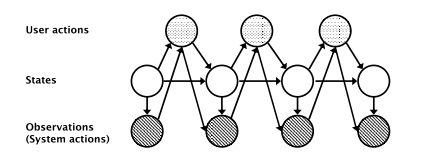
\includegraphics[width=.6\linewidth]{khan2004-hmm.png}\\
  \caption{An example of the HMM approach}\label{fig:khan04-hmm}
\end{figure}

\textbf{Hidden Markov Models} In the work of \cite{Cuayahuitl2005}, the authors experiment with different variations of HMMs, and show that the most advanced one is an \emph{Input-Output-HMM (IOHMM)}  (cf. Figure \ref{fig:khan04-hmm}). The behaviour of the model is governed by a set of transition probabilities $P(q_{t+1} | q_t, a_{u,t})$ and a set of output probabilities $P(a_{s,t} | q_t, a_{u, t-1})$. User responses are predicted using $P(a_{u,t} | q_t, a_{s,t})$.

Finally the paper introduces some evaluation techniques, in which a distinction can be made between \emph{direct} methods and \emph{indirect} methods. Direct evaluation methods assess the user model by testing the quality of its predictions, such as accuracy, precision and recall. Indirect evaluation metrics such as utility attempt to measure the quality by evaluating the effect on the system performance.
